\documentclass[fleqn,a4paper,12pt,oneside]{article}
\usepackage{graphicx}
\usepackage{float}
\usepackage{amsmath}
\usepackage{amsfonts}
\usepackage{amssymb}
\usepackage[table]{xcolor}
\usepackage[left = 1.5in, right = 2.5cm, top = 2.5cm, bottom = 2.5cm]{geometry}
\usepackage[font = footnotesize, labelfont = bf]{caption}

\begin{document}
	\title{\bf STUDY OF AMBIENT INTERSTELLAR MEDIUM AND ASYMPTOTIC GIANT BRANCH STARS AT DIFFERENT LATITUDES}
	\author{\textbf{A Research Proposal}
		\\
		\\
		Submitted  to the University Grants Commision,\\Research Division,\\Sanothimi, Bhaktapur, Nepal\\ 
		For the UGC Small RDI Grant 
		\\
		\\
		{
\includegraphics[width=2cm]{logo}}
		\\
		\\
		By}
	\vspace{1cm}
	\date{\bf Devendra Raj Upadhyay\\Lecturer\\ Amrit Campus, Tribhuvan University, \\Kathmandu, Nepal\\\vspace{1cm}\today}
	\setlength{\textheight}{23.5cm} \maketitle
	\setlength{\textheight}{23cm}
	%------------------------------------------------------
	\clearpage
	\pagenumbering{roman}
	
	\tableofcontents
	\pagebreak
	\pagenumbering{arabic}
\section{Purpose}
 The proposed research work is entitled {\bf``STUDY OF AMBIENT INTERSTELLAR MEDIUM AND ASYMPTOTIC GIANT BRANCH STARS AT DIFFERENT LATITUDES''.}
\section{Abstract}
In this research work we will discuss how different physical parameters like flux, temperature, mass
distributed near low intermediate mass star (0.8 - 8 M$_{\odot}$; LIMS) i.e. Asymptotic Giant Branch (AGB) stars. AGB stars are very
important contributors of material to the interstellar medium
(ISM), and yet the mechanisms by which this matter is expelled
remain a mystery, temperature profile, shock nature of
AGB star near cavity like structure plays a role in studying the
interaction between ISM and AGB star at  different latitudes. We will study using modern technologies and programs for the investigation different properties around AGB stars. 
\section{ Background/Context/Problem}
  The interstellar medium in the vicinity of the Sun is arranged in
large scale structures of bubble walls, sheets, and filaments of
warm gas, within which close to the mid plane there are sub-sheets
and filaments of cold dense material; the whole occupies roughly
half the available volume and extends with decreasing mean density
to at least a kilo parsec off the plane. The remainder of the
volume is in bubble interiors, cavities, and tunnels of much lower
density, with some but not all of those lower density regions hot
enough to be observable via their X-ray emission. This entire
system is pervaded by a rather strong and irregular magnetic field
and cosmic rays, the pressures of which are confined by the weight
of the interstellar gas, particularly that far from the plane
where gravity is strong \cite{4}. In thermodynamic equilibrium, a
medium is characterized by a single temperature, which describes
the velocity distribution, excitation, ionization, and molecular
composition of the gas. While the velocity distribution of the gas
can generally be well described by a single temperature, the
excitation, ionization, and molecular composition are often very
different from thermodynamic equilibrium values at this
temperature. This reflects the low pressure of the ISM, so that,
for example, collisions cannot keep up with the fast radiative
decay rates of atomic and molecular levels. Ionization and
chemical composition are also kept from their equilibrium values
by the presence of $\sim$100 MeV cosmic-ray particles clearly a
non-Maxwellian component and a diluted, stellar, EUV(10-124 nm) -
FUV (100-200 nm) photon field, which is much stronger than a 100 K
medium would normally have. Finally, the large-scale velocity
field is much influenced by the input of mechanical energy.
Whenever a gas is not in local thermodynamic equilibrium, the
level populations, degree of ionization, chemical composition, and
of course the temperature are set by balancing the rates of the
processes involved. Much of the study of the ISM is thus concerned
with identifying the various processes that control the ionization
and energy balance, setting up the detailed statistical
equilibrium equations and solving them for the conditions
appropriate for the medium \cite{5}.
\\
\\
We intend to search suitable condition so that the interaction
between AGB wind and ISM can be studied. In this research work we
are focused on the how C-rich AGB star show behavior around their
surroundings.
Following are the valid problems of research
\begin{itemize}
	\item  It is believed that the shaping of infrared dust structure
has a close relation with the inhomogeneous Interstellar Medium
(ISM). The violent stellar phenomena lead inhomogeneity in the
ISM. We intend to perform a multi wavelength study in the
far infrared emission region. This may reveal the presence and
role of hot phenomena (X-rays, gamma rays, etc) in the shaping
process. \item  A  far infrared loops around ATNF Pulsars studied by A. K. Jha,  B. Aryal \& R. Weinberger (2017). There is lack of study such type of phenomenon in AGB star so I intend to study similar phenomena in AGB stars \cite{akj}.  
\item Asymmetry mass ejection during the AGB phase was concluded
by Zijlstra \& Weinberger (2002), Aryal \& Weinberger (2006), Aryal, Rajbahak \& Weinberger
(2009), Aryal, Rajbahak \& Weinberger (2010) by studying dust
structures around planetary nebula \cite{B_1,B_2,B_4}.
\end{itemize}


%------------------------------------------------------

%------------------------------------------------------
\section{Literature Review}
\subsection{Interaction between ISM and the Stellar Wind}Many theoretical studies predict that the interaction of suitable
stellar wind with the interstellar medium (ISM) creates
``Interstellar Bubbles". One of the model  proposed by Weaver $et$ $al$. (1977)
regarding the existence of interstellar bubble due to the
interaction between stellar wind and homogeneous interstellar
medium. Most of the theory presented below concerns with the
following idealized model. At time t = 0, an early type star
begins to blow a steady, spherically symmetric stellar wind with
constant terminal velocity $V_{w}$ and mass loss rate $dM_{w}/dt$.
The mechanical luminosity of $L_{w}$ of the wind is therefore
given by
\begin{equation}\label{1}
L_{w} ={\frac{1}{2}\frac{dM_w}{dt}V^{2}_{w}}
\end{equation}
This wind interacts with an ambient interstellar gas of uniform
atomic density $n_{0}$ and given cosmic abundances, resulting in
an expanding spherical system, which we shall call a bubble.
Throughout it's evolution, the dynamical system consists of four
distinct zones. Starting from within, they are: (a) the hypersonic
stellar wind: (b) a region of shocked stellar wind: (c) a shell of
shocked interstellar gas: and (d) ambient interstellar gas. This
structure is depicted schematically in Fig. (1) \cite{10}.
%\begin{figure}[h]
%	\centering
%	% Requires \usepackage{graphicx}
%	\includegraphics[width =10cm]{Shock}
%	\caption{A schematic diagram of the various regions created by the stellar
%		wind from a massive star. $R_{1}$ is the location of the wind
%		shock, $R_{2}$ is the location of the shock in the ambient medium,
%		and $R_{c}$ is the location of the contact discontinuity. Here the
%		shell of shocked interstellar gas is cool and thin, while the
%		shocked stellar wind is hot and tenuous. The sizes of the
%		different regions are thus not to scale \cite{10}.}\label{Figure}
%\end{figure}
\\
The evolutionary history of the bubble may be divided into three
stages. At first, the bubble is expanding so fast that radiative
losses in the gas do not have time to affect any part of the
system, and the dynamics of each region is described by adiabatic
flow. In the second stage, radiative losses cause the expanding
shell of swept-up interstellar gas in region (c) to collapse into
a thin shell; but region (b), the shocked stellar wind, still
conserves energy. In the final stage, the radiative losses also
affect the dynamics of region (b).
\\
\\
The structure of bubble during the first stage and the
transition from  first stage to the second stage have been
considered by V. S. Avedisova  and by S. A. E. G. Falle. They show
that the first stage lasts a very short time; therefore, the
structure during this first stage is of of somewhat academic
interest. However, Weaver $et$ $al$. shall review the problem
since  above discussions are not complete, and since the
hydrodynamical solutions obtain may apply to a broader context
than just the present model of a stellar wind interacting with
interstellar gas. It is assumed that first region (c) of
swept-up interstellar gas, whose outer boundary, at R$_{2}$, is
a shock separating it from the ambient interstellar gas (d), and
whose inner boundary, at R$_{c}$, is a contact discontinuity
separating it from the shocked stellar wind (b). The structure
of the region can be described by similarity solution.
Here the theory of the adiabatic blast wave given by Weaver $et$ $al.$\cite{10} assumed that the energy is
fed into the system at a constant rate instead of in an initial
blast \cite{10}.
\\\\
Weaver $et$ $al$. (1977) neglecting gravity assumed that the flow is spherically
symmetric, and find the equations of motion and
continuity are equations describes the dynamics of  interstellar
medium can be described by the continuity, momentum, and energy
equations \cite{10}.






\subsection{Inhomogeneity}
Segregation of the matter into cold and warm components is not the
only source of inhomogeneity in the ISM. In this section we
consider the arm$/$interarm contrast, the observations indicating
that there are large cavities and tunnels of very low density in
the ISM and  observed distribution of the denser matter. The
interstellar medium is expected to have a certain amount of
large-scale inhomogeneity just from dynamical events \cite{4}.
\\
\\
To study the properties such as inhomogeneity of ISM and AGB wind we must define
some of the terms like source term in R.H.S. of expression.
Without neglecting gravity and we assume that the flow is
asymmetric, the equations of motion is inhomogeneous and
discontinuity. This term is either defined as four dimensional
tensor which includes space and time both or simply impulse as:
\begin{equation}\label{1}
\frac{{\partial}{v}}{{\partial}t} +
{v}\frac{{\partial}v}{{\partial}r} +
\frac{1}{\rho}\frac{{\partial}p}{{\partial}r}= f(r, t),
\end{equation}
and
\begin{equation}\label{2}
\frac{{\partial}{\rho}}{{\partial}t} +
v\frac{{\partial}\rho}{{\partial}r}+
\rho\frac{{\partial}v}{{\partial}r}+ 2\frac{{\rho}v}{r} = f(r, t).
\end{equation}
The equation of energy conservation for the adiabatic flow during
this stage is
\begin{equation}\label{3}
\frac{D}{Dt}(p{\rho}^{-\gamma}) = f(r, t),
\end{equation}
Where,
\\ $\frac{D}{Dt} = \frac{\partial}{{\partial}t} + {v}\frac{\partial}{{\partial}r}$
and $\gamma = \frac{5}{3}$, the equation of energy conservation
for the adiabatic flow may other types of flow there during this
stage equation can be written is in the form
\begin{equation}\label{4}
\frac{ D}{Dt}(p{\rho}^{-\gamma}) = f(r,t),
\end{equation}
Where, \\
$\frac{ D}{Dt} = \frac{\partial}{{\partial}t} +
{v}\frac{\partial}{{\partial}r}$ and $\gamma = \frac{5}{3}$.\\
\\As the equation
\begin{equation}\label{1}
{\Box_{x,t}^2}\Psi(\vec{X},t) = f(\vec{X} ,t)
\end{equation}
Where, ${\Box_{x,t}^2} = \nabla^{2} -
\frac{1}{c^2}\frac{{\partial}^2}{{\partial}t^2}$ is called is
D'Alembertian. We wish to solve the equation
\begin{equation}
(\nabla^{2} - \frac{1}{c^2}\frac{{\partial}^2}{{\partial}t^2})G(\textbf{X}-\textbf{X}',
t-t') =
- {\delta}(\textbf{X}-\textbf{X}', t-t')\delta(t - t')
\end{equation}
Where, $G(\textbf{X}-\textbf{X}', t-t')$ is the solution of
equation (7) and $\delta(\textbf{X}-\textbf{X}')$ = $\delta(x -
x')\delta(y - y')\delta(z -z')$ is called Dirac Delta function and
The mathematical detailed is not mentioned here but in shortly the
solution of equation (7):
\begin{equation}
G(\textbf{X}-\textbf{X}') = - \frac{c}{4{\pi}|\textbf{X} -
	\textbf{X}|}[\delta[(|\textbf{X}-\textbf{X}'| - c(t - t')] -
\delta[(|\textbf{X}-\textbf{X}'| + c(t - t')]
\end{equation}
Here, the Green's function with first delta function, i.e.,
\begin{equation}
G(\textbf{X}-\textbf{X}') = - \frac{c}{4{\pi}|\textbf{X} -
	\textbf{X}|}\delta[(|\textbf{X}-\textbf{X}'| - c(t - t')]
\end{equation}
is called the retarded or causal Green's function because the
source point time $t'$ is always earlier than the observation
point time $t$ which describes how causality is conserved, i.e.
effect after cause and used for positive time particle. The
Green's function
\begin{equation}
G(\textbf{X}-\textbf{X}') =  \frac{c}{4{\pi}|\textbf{X} -
	\textbf{X}|}\delta[(|\textbf{X}-\textbf{X}'| + c(t - t')]
\end{equation} is called advanced Green's function which violets
causality, i.e., effect before cause and used for negative time
particle called antiparticle.
\\In similar manner in electromagnetic field
\begin{equation}\label{1}
{{\partial}_{\alpha}}F^{\alpha\beta}=\frac{4\pi}{c} J^{\beta}
\end{equation}
With the definition of the fields in terms of the potentials this
becomes
\begin{equation}\label{1}
{\Box}A^{\beta} - \partial^{\beta}(\partial_{\alpha}A^{\beta}) =
\frac{4\pi}{c}J^{\beta}
\end{equation}
If the potential satisfy the Lorentz condition,
${\partial}_{\alpha}A^{\beta}$ = 0, the four-dimensional wave
equation in covariant form: \begin{equation}\label{1}
{\Box}A^{\beta} = \frac{4\pi}{c}J^{\beta}
\end{equation}
Using Green function method we intended to solve many
inhomogeneous issues encounter in interstellar medium. The
differential equations encountered in physical problems are not
always homogeneous.\cite{14} If either the differential equation
or boundary conditions or both are non-homogeneous, the boundary
value problem is called non-homogeneous. The method of Green's
function is convenient technique for such problems. In 1828 George
Green (1793 - 1841) published an essay on the application of
mathematical Analysis to the theory of Electricity and magnetism.
In this seminal work of mathematical physics, Green sought to
determine electric potential with in a vacuum bounded by
conductors with specified potentials \cite{G}. Here in ISM and AGB
wind interaction case there is also the asymmetry, i.e., symmetry
breaking also the ISM is not in LTE (Local thermodynamic Equilibrium) which violates the symmetry and LTE. In our region
of interest there is huge variation of density near the cavity
there is less dense which disturb the LTE.



\subsection{Ambient Interstellar Medium}
The interstellar medium in the vicinity of the Sun is arranged in
large-scale structures of bubble walls, sheets, and filaments of
warm gas, within which close to the mid-plane there are sub sheets
and filaments of cold dense material; the whole occupies roughly
half the available volume and extends with decreasing mean density
to at least a kilo parsec off the plane. The remainder of volume is in bubble interiors, cavities, and tunnels of much lower
density, with some but not all of those lower density regions hot
enough to be observable via their X-ray emission. This entire
system is pervaded by a rather strong and irregular magnetic field
and cosmic rays, the pressures of which are confined by the weight
of the interstellar gas, particularly that far from the plane
where gravity is strong. Observations suggest that the cosmic rays
and magnetic field have an even more extended vertical
distribution than the warm gas, requiring either the weight of
additional coronal material or magnetic tension  confine it to
the disk. Adjusting one's perception of this medium to embrace the
known aspects is difficult. After this adjustment, there are many
problems to solve and prejudices to overcome the weak role of
thermal instability, the suppression of certain gravitational
instabilities, the problem of determining the state in a
low-density regions, the twin difficulties of not having too much
OVI $(O^{+5})$ and getting enough diffuse 3/4 KeV, X-ray emission,
the possible importance of large old-barrel shaped supernova
remnants in clarifying matters, the possible role of dust
evolution in adjusting the heating to make clouds stable, the
factors influencing the magnitudes of the interstellar pressure
and scale height things that global models of the medium might
examine to clarify some of these matters; attention to these
details and more constitute the challenge of this subject.



\subsection{Asymptotic Giant Branch Phase}
Our knowledge of the AGB phase of evolution has increased
dramatically over the last  2 decade or so, driven primarily by
observations. Theoretical studies are desperately needed to
quantify the nucleosynthesis which occurs in intermediate mass
stars during their thermally pulsing evolution. A period of
stellar evolution undertaken by all low to intermediate mass stars
(0.8 - 8 solar masses) late in their life is called Asymptotic
Giant Branch (AGB) phase. The structure of a star when it reaches
the AGB is characterized by: (i) a small, very hot and dense core
of carbon and oxygen; (ii) He- and H- alternately burning shells;
(iii) a large, hot, and less dense stellar envelope; (vi) a warm
atmosphere and a very large, diluted and cool circumstellar
envelope. for stars with masses between about 1 and 8 M$_{\odot}$
the ascent of the AGB is the last nuclear powered evolutionary
stage. Although only short in duration, the AGB is very important
due to the nucleosynthesis which occurs.
\\
  The
asymptotic giant branch (AGB) is the region of the
Hertzsprung-Russell diagram populated by evolving low- to
medium-mass stars. This is a period of stellar evolution
undertaken by all low- to intermediate-mass stars (0.6 - 10)
M$_{\odot}$ late in their lives. Asymptotic giant branch (AGB)
stars are generally classified as oxygen-rich (M-type) or
carbon-rich (C-type) based on the chemistry of the photosphere and
or the outer envelope \cite{1}.



\section{ Theoretical/Technical Aspect}
\subsection{Dust Color Temperature Estimation}
There are many model for calculation of temperature with the help
of different data base. In this sort of dissertation work we use
data base from the IRAS 60 $\mu$m and 100 $\mu$m flux densities is
similar to that of Schnee $et$ $al.$ (2005) \cite{36}. By knowing
the flux densities at 60 $\mu$m and 100 $\mu$m, the temperature
contribution due to dust color can be calculated. The dust
temperature $T_{d}$ in each pixel of a FITS (Flexible Image
Transport System) image can be obtained by assuming that the dust
in a single beam is isothermal and that the observed ratio of 60
$\mu$m to 100 $\mu$m emission is due to black body radiation from
dust grains at $T_{d}$, modified by a power law of spectral
emissivity index. The flux density of emission at a wavelength
$\lambda_{i}$ is given by
\begin{equation}\label{3}
F_{i} = \bigg[\frac{2hc}{\lambda^{3}_{i}(e^{\frac{hc}{\lambda_{i}KT_{d}}}-1)}\bigg]N_{d}\alpha\lambda_{i}^{-\beta}\Omega_{i}
\end{equation}
where, $N_{d}$ is the column density of dust grains, $\alpha$ is a
constant which relates the flux with the optical depth of the
dust, $\beta$ is the spectral emissivity index, and $\Omega_{i}$
is the solid angle subtended at $\lambda_{i}$ by the detector.
Following Dupac $et$ $al.$ (2003)\cite{37}, we use the equation
\begin{equation}\label{4}
\beta = \frac{1}{(\delta+wT_{d})}
\end{equation}
to describe the observed inverse relationship between temperature
and emissivity spectral index. Here, $\delta$ and $\omega$ are fee
parameters found that the temperature dependence of the emissivity
index fits very well with the hyperbolic approximating
function \cite{37}.
\\Considering temperature as an independent variable, the best fit gives
$\delta$ = 0.40 $\pm$ 0.02 and $\omega$ = 0.0079 $\pm$ 0.0005 K$^{-1}$, with
the $\chi^{2}/$degree of freedom = 120/120. With the assumptions that the dust emission is optically thin at
60 $\mu$m and 100 $\mu$m and that $\Omega_{\omega}$$\simeq$
$\Omega_{100}$ (true for IRAS image), we can write the ratio, R,
of the flux densities at 60 $\mu$m and 100 $\mu$m as
\begin{equation}\label{5}
R =  0.6^{-(3+\beta)}\bigg[\frac{e^{\frac{144}{T_{d}}}-1}{e^{\frac{240}{T_{d}}}-1}\bigg]
\end{equation}
The value of $\beta$ depends on dust grain properties as
composition, size, and compactness. For reference, a pure
blackbody would have $\beta$ = 0, the amorphous layer-lattice
matter has $\beta \sim 1$, and the metals and
crystalline dielectrics have $\beta \sim 2$.\\
\\
For a smaller value of $T_{d}$, 1 can be dropped from both
numerator and denominator of equation (16) and it takes the form
\begin{equation}\label{6}
R =
0.6^{-(3+\beta)}\bigg[\frac{e^{\frac{144}{T_{d}}}}{e^{\frac{240}{T_{d}}}}\bigg]
\end{equation}
Taking natural logarithm on both sides of equation (2.50) we find
the expression for the temperature as
\begin{equation}\label{7}
T_{d} = \frac{-96}{ln\{R \times 0.6^{(3+\beta)}\}}
\end{equation}
where R is given by
\begin{equation}\label{8}
R = \frac{F(60 \mu m)}{F(100 \mu m)}
\end{equation}
F(60 $\mu$m) and F(100 $\mu$m) are the flux densities at 60 $\mu$m
and 100 $\mu$m, respectively. In this way we can use equation
(18) for the determination of the dust grain temperature.
\subsection{Mass Estimation}
Since the longer wavelength measurements give us more precise dust
masses due to the characteristics of  Planck curve, the far
infrared emission which is used for the derivation of  dust
mass is measured from the 100 $\mu$m IRAS images.  The dust masses
are estimated from the IR flux densities \cite{38}.
\\
\\
In order to estimate the dust masses from the infrared flux
densities at 100 $\mu$m, following the calculation of Young $et$
$al.$\cite{39} we need the background correction of flux and
convert the relative flux into absolute flux. The background
correction is done by subtracting the average flux emitted by the
external sources other than the object of interest. The black body
intensity can be calculated using the basic expression as given in
equation (22). The resulting dust mass depends on the physical
and chemical properties of the dust grains, the adopted dust
temperature $T$ and the distance $D$ to the object.
\begin{equation}\label{9}
M_{dust} = \frac{4}{{3}}\frac{a\rho}{{Q_{\nu}}}\bigg[\frac{S_{\nu}D^{2}}{{B(\nu, T)}}\bigg]
\end{equation}
where,\\
$a$ = weighted grain size\\
$\rho$ = grain density \\
$D$ = Distance to the star\\
$ Q_{\nu}$ = grain emissivity\\
$ S_{\nu}$ = f $\times$ MJy/Sr $\times$ 5.288 $\times$ 10$^{-9}$
\\
\\
\textbf{For 100 $\mu$m emitter}
\\
$a$ = 0.1 $\mu$m\\
$\rho$ = grain density =3000 kg m$^{3}$ ,
Q$_{\nu}$ = grain emissivity = 0.0010 (for 100 $\mu$m)\\
Q$_{\nu}$ = grain emissivity = 0.0046 (for 60 $\mu$m)
\cite{39}\\
$ S_{\nu}$ = f $\times$ MJy/Sr $\times$ 5.288 $\times$ 10$^{-9}$\\
where, 1 MJy/Sr = 1 $\times 10^{-20}$ kg s$^{-2}$ and f = relative
flux density measured from the Groningen IRAS image\cite{41}.\\
For 100 $\mu$m wavelength, the expression for the dust mass
reduces to,
\begin{equation}\label{9}
M_{dust} = 0.40\bigg[\frac{S_{\nu}D^{2}}{{B(\nu, T)}}\bigg]
\end{equation}
The Planck's function is a well known function, given by this
equation,
\begin{equation}\label{10}
B(\nu, T) = \frac{2h\nu^{3}}{{c^{2}}}\bigg[\frac{1}{exp^(\frac{h\nu}{KT})-1}\bigg]
\end{equation}
Where,
\\
$h$ = Planck's constant\\
$c$ = velocity of light\\
${\nu}$ = frequency at which the emission is observed\\
$T$ = Temperature of each pixel
\\
\\
It is clear from the expression (22) that the value of Planck
function B ($\nu$, T) for longer wavelength is higher than that of
the shorter wavelength. Consequently, the range of B ($\nu$, T)
for fixed temperature (say $\Delta$T) goes narrower if wavelength
of the images increases \cite{39}.
\section{Significance of the Development/Innovation}
An interesting result obtained by  Jha $et$ $al.$ (2017) from the study of far infrared loop-like structures (KK-loops) in 100 and 60 $\mu$m IRAS maps which are identified by Kiss et al. (2004) and Koenyves et al. (2007). They reported 462 far infrared loops. In the study of  KK-loop G007+18 is 2.2$^{\circ}$ $\times$
2.1$^{\circ}$ (Koenyves et al. 2007) whereas its core size is
0.9$^{\circ}$ $\times$ 0.4$^{\circ}$. Therefore the core region of
this loop is only $\sim$ 8\% of the whole loop. An extended
principle minima can be seen in the central region (Fig. 2 a). The
dust color temperature (T$_{d}$ hereafter) calculated using the
slope of $F$(100) and $F$(60) plot (Fig. 2 b) is found to be
minimum, i.e., 20.1$\pm$1.1K. The minimum and maximum value of
T$_{d}$ is found to lie in the range 19.1$\pm$1.1K and
20.8$\pm$1.2K. An offset of $<$ 2K suggests that the core of the
loop is stable. The minimum temperature region is found to be
elongated along north-south direction (Fig. 2 c). The dust mass
contours (Fig. 2 d) seem to follow the expected trend: higher
density at low temperature region.
%\begin{figure}[h]
%	\vspace{0cm} \centering
%	\includegraphics[height=4.5cm]{G007a.eps}
%	\includegraphics[height=4.5cm]{G007b.eps}
%	\includegraphics[height=4.5cm]{G007c.eps}
%	\includegraphics[height=4.5cm]{G007d.eps}
%	\includegraphics[height=4.7cm]{G007e.eps}
%	\includegraphics[height=4.7cm]{G007f.eps}
%	\caption[]{(a) IRIS 100 $\mu$m far infrared images of the core
%		region of KK-loop G007+18 centered at (a) RA (J2000) =
%		17$^{h}$00$^{m}$5.4$^{s}$, Dec (J2000) = $-$11$^{\circ}$55'51.2".
%		The contours and image size are shown. The IRAS contour represent
%		19.2, 19.6, 19.9, 20.3, 20.7, 21.1, 21.5 and 21.9 MJy sr$^{-1}$.
%		(b) Flux at 100 $\mu$m versus 60 $\mu$m plot. The dust color
%		temperature (c) and dust mass (d) contour maps. The contour levels
%		are shown. The distribution of dust color temperature (e) and dust
%		mass (f). The solid curve represents Gaussian fits. The Gaussian
%		parameters are given \cite{akj}.}
%\end{figure}
The distribution of dust color temperature fits well with Gaussian
(Fig. 2 e) with Gaussian center at 19.9K. The value of T$_{d}$ of
the larger structure is found to be 33.0$\pm$2.1K. Therefore the
cavity is cold (low density) enough at the core region than that
of the outer region. As a whole, an offset of 15 K temperature
suggest that the cavity is dynamically active. The inclination
angle of its core (area $\sim$ 0.36 square degree) is found to be
83$^{\circ}$ (edge-on) whereas it is 25$^{\circ}$ (face-on) as a
whole (area $\sim$ 4.6 square degree). Jha $et$ $al$.(2017) concluded that the inner region
of KK-loop G007+18 is found to be oriented by about
58$\sim$60$^{\circ}$ (assuming the loop is in the sky plane). It
means that our dusty loop is neither face-on ($i$ $\rightarrow$
0$^{\circ}$) nor edge-on ($i$ $\rightarrow$ 90$^{\circ}$) \cite{akj}.
\\
Another result obtained by  Aryal $et$ $al.$ (2010)
suggested that different structures described are physically
related to NGC 1514 and can be put in chronological order: the
roundish nebula is the fossil remnant of the spherically symmetric
outflow in the AGB phase. The outer bipolar structure marks the
first (massive) aspherical outflow in the PPN phase, later
followed by a second one (the inner bipolar structure), which took
place along an other axis due to precision. Later, the PN formed
and was partly shaped by the effects of the earlier dusty outflows
as indicated by its brightness depression along the same axis as
the inner bipolar structure. These collimated outflows could have
been driven by the hot compact central star. To sum up, NGC 1514
and its surroundings could represent the preserved history of the
main mass-loss phases of a star of intermediate initial
mass \cite{B_4}.
%\begin{figure}[h]
%	\vspace{0.0cm} \centering
%	\includegraphics[height=4cm]{PN}
%	\includegraphics[height=4cm]{BA}
%	\caption{Left: Optical image of the PN NGC 1514\cite{13}. At the
%		nebula's center, there is the bright A0III star HD 281679, the
%		companion star of the spectroscopically confirmed Seaton (1980)
%		hot ($\sim6\times10^{4}$ K) central star. North is up, east to the
%		left. Note the brightness depression in the nebula and the faint
%		protrusion of nebular emission towards the south-west, at a
%		position angle PA $\sim 197^{\circ} \pm 5^{\circ}$. Right: Contour
%		map of a $\sim$1$^{\circ}$ $\times$ 1$^{\circ}$ region at 100
%		$\mu$m centered on NGC 1514 \cite{B_4}.}
%\end{figure}
\\
\\
Aryal $et$ $al$. (2010) mentioned in paper Typical wind velocities
in the AGB phase are 10 - 20 km s$^{-1}$. To cover the angular
distance of $0.4^{\circ}$ (i.e. 1.29 pc at D = 185 pc) with a
constant velocity of 15 km s$^{-1}$ takes 8.4 $\times$ $10^{4}$
years. In this way it is concluded that  this is approximately the
time when the strong spherical AGB mass loss started; its material
is now visible as the roundish nebula of dust emission. In the
short (typically $\sim$ 1000 years) phase of transformation from
spherical mass loss into an aspherical nebula, the outer structure
(A - A') in Fig. 2A was generated; it may contain entrained
material from the AGB wind \cite{B_4}.
\section{Foundational/ Preliminary Work} 
I have supervised two M.Sc. Project Works related to AGB stars and nine B.Sc.Project Works related to AGB stars, Nebulae and Moon Craters.
Now five B.Sc.Project Works, two M.Sc. project works and one M.Sc. thesis with collaborations and myself are in pipeline. I hope this grant strengthen our research works. 

\section{Development/Innovation Goal/ Objectives} 
After the completion of  research work, it is expected to discover cavity or nebular like structures. Further, dust color temperature,  intensity variation and mass profile of the structure will be studied. The interaction between different AGB stars in  interstellar medium will be studied. We also interested to interpret different shock wave ejected by far infrared loops wind with inhomogeneous nature and want to introduce Green’s function technique for solving such problem. The research will be submitted to the University Grants Commission, Sanothimi Bhaktapur, Nepal.
\begin{itemize}
\item {\bf{Quality Education:}} We realized the need of this research as we found most of our under-graduate and graduate students lacking in  research skills which is needed for their career in science and physics. We believe, it will be able to help our undergraduate and graduate students to develop their research skills at the end of  research work.
\item {\bf Gender Equality:} Few  female students are interested to do research in Astrophysics and Astronomy in our departments and hence this grant help us and them to provide  more access towards research opportunities in Nepal.
\item {\bf Innovation:} We believe the computational skills we will develop during the research help us and students become innovative and think of more research engagement in future.
\end{itemize}
Following are the  major objectives of this
work:
\begin{itemize} 
	\item To investigate the new isolated cavity structure including cavity in
	IRAS, IRIS, AKARI and 2MASS maps by performing a systematic search in all wavelength
	band in the these surveys of C-rich, O-rich and  Si- rich AGB stars catalog.
	\item To know the model of cavity formation due to AGB wind, we intend to study the flux density, dust color temperature, intensity variation, dust-grain mass distribution, outflow nature and associated energy of the structure.
	\item To estimate Shock nature, i.e., C-shock and J-shock\cite{5} ejected by AGB
	wind. By knowing inhomogeneous nature of medium we will try to
	correlate or interpret in term of Green's function technique.
\end{itemize}
\section{Design / Methodology and Verification }
\subsection{Research design}
We are planing to perform this research  with the help of data provided by Infrared Astronomical Satellite Survey(IRAS), Improved Reprocessing of the IRAS Survey (IRIS), AKARI and 2MASS data using Set of Identifications, Measurements and Bibliography for Astronomical Data (SIMBAD) \cite{34,35}. We have plan to conduct this research work at computational laboratory of Amrit Cam-
pus, Thamel, Kathmandu, Nepal. So, the fund provided will be used to upgrade the
computer system provided in Amrit Campus, Thamel, Kathmandu Nepal at computa-
tional laboratory. Data will be processed by using Aladin, Python, Origin, and Octave
softwares among which we plan to buy with the fund provided to us. We will adopt
following procedures in order to carry out proposed work:
%\begin{figure}[h!]
%	\centering
%	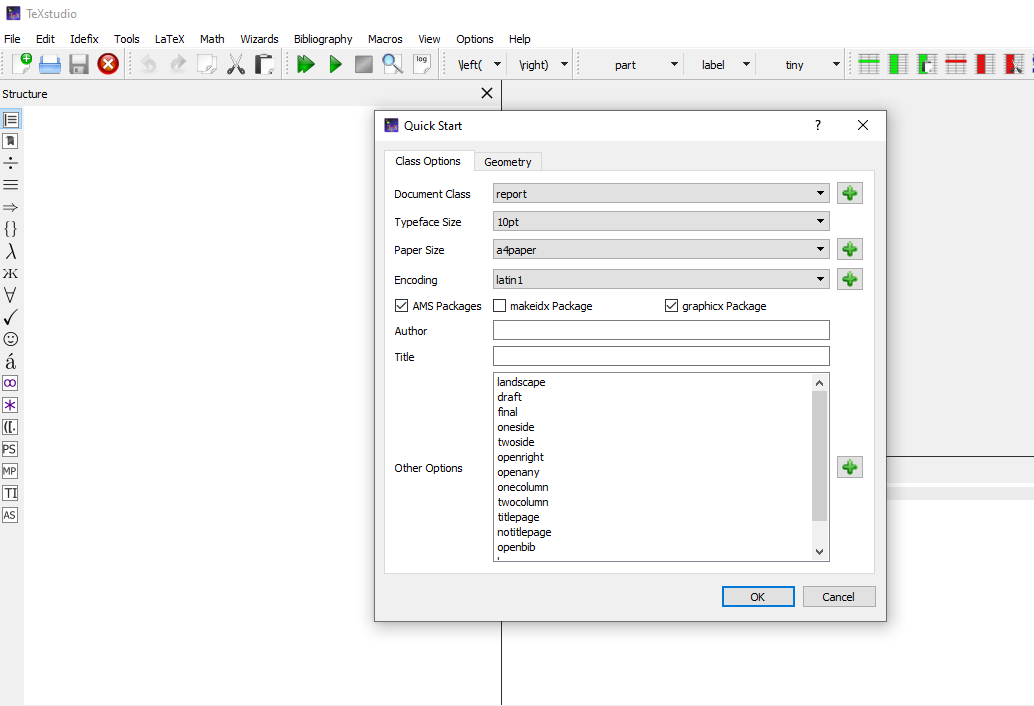
\includegraphics[width=12cm]{1.PNG}
%	\caption{The flow chart of the procedure and data analysis plan.}
%\end{figure}
\subsection{Infrared Astronomical Satellite Survey}
IRAS was a joint project of the US, UK and the Netherlands.  For ten months in 1983, the Infrared Astronomical
Satellite (IRAS) scanned more than 96 $\%$ of the sky.
 IRAS discoveries included a disk of dust grains around the star
Vega, six new comets, and very strong infrared emission from
interacting galaxies as well as wisps of warm dust called infrared
cirrus which could be found in almost every direction of space.
%\begin{figure}[h!]
%	\vspace{0.0cm} \centering
%	\includegraphics[height=5cm]{IRAS1}
%	\includegraphics[height=5cm]{IRAS}
%	\caption{Left: The Infrared Astronomical Satellite (IRAS)
%		\cite{32}. Right: The Infrared Astronomical Satellite (IRAS)
%		during the magnetic moment test conducted in The Netherlands. The
%		satellite was slowly spun and the variations to the magnetic field
%		were measured \cite{33}.}
%\end{figure}
IRAS also revealed for the first time the core of our galaxy, the
Milky Way. 
\\
Aladin v2.5 and Aladin v9 are an interactive sky atlas developed and maintained by the Center deDonne's astronomiques de Strasbourg (CDS) for the identification
of astronomical sources through visual analysis of reference sky
images. Aladin v2.5 and Aladin v9 allows the user to visualize digitized images
of any part of the sky, to superimpose entries from the CDS
astronomical catalogs and tables, and to interactively access
related data and information from SIMBAD, NED or other archives of
all known objects in the field.
\subsection{Spitzer Survey Telescope}
The Spitzer Space Telescope was launched on August 25, 2003. Spitzer is the final mission in NASA's Great Observatories Program. During the 5.5 year cryogenic mission, Spitzer made spectral and photometric observations between wavelengths of 3 and 180 microns. Imaging at 3.6 and 4.5 microns continues during the ongoing Spitzer Warm Mission. IRSA serves all Spitzer data from both the cryogenic and warm missions through the Spitzer Heritage Archive (SHA). In addition, IRSA serves enhanced data products from Spitzer Legacy programs.   
%\begin{figure}[h!]
%	\vspace{0.0cm} \centering
%	\includegraphics[height=4.5cm]{spitzer.jpg}
%	\includegraphics[height=4.5cm]{1s.jpg}
%	\caption{Left: The Spitzer Space Telescope is designed to detect infrared radiation, which is primarily heat radiation, allowing scientists to examine cosmic regions that are hidden from optical telescopes such as dusty stellar nurseries, the centers of galaxies, and newly formed planetary systems.\cite{L} Right: This artist's concept shows Spitzer surrounded by examples of exoplanets the telescope has examined \cite{R}.}
%\end{figure}

%\section{Population and sample}
%In the collection of sample I am planing to  follow the SIMBAD database, Sky View Virtual Observatory.
%I have a catalog of AGB stars (version. 2011)
%Suh $\&$ Kwon (2011) which present a catalog of AGB stars for 3003 O-rich, 1168 C-rich, 362 S-type and 35 silicate carbon stars in
%our Galaxy which is a revised version of the catalog of AGB stars
%Suh $et$ $al.$ by (2009)\cite{29} presented a catalog of AGB stars in
%our Galaxy from the sources listed in the IRAS PSC compiling the
%lists of previous works with verifying processes; their catalog
%was made of 2193 O-rich stars, 1167 C-rich stars, 287 S stars and
%36 silicate carbon stars.\cite{30} Kwon \& Suh (2012) presented a revised sample of 3373 O-rich AGB stars.
%Again Kwon \& Suh (2014) presented a more revised catalog of 29 silicate carbon stars, from which two of them are post-AGB stars. Finally Suh \& Hong (2017) presented a revised catalog of 3828 O-rich AGB stars and 1168 C-rich AGB stars excluding misclassified objects (O-rich: 15, C-rich: 9) and adding newly identified objects (O-rich: 470, C-rich: 9). Above mentioned are the source of data and sample. The updated catalogue data will
%be open to the public through the first author's world wide web
%site at mentioned link \cite{30,ns}. 
% \section{Expected Findings}

\section{Expected Product}
Our  research interests lie in astronomy and astrophysics. We have a
small group continuously working on several topic. Basically our
researches concern about the ``STUDY OF INTERSTELLAR MEDIUM AND ASYMPTOTIC GIANT BRANCH STARS AT DIFFERENT LATITUDES'' and main focus of this project is to motivate students for research activities.
The major expected output of this project will be as follows:
\begin{itemize}
\item I will supervise at least one Master student and two bachelors students (project works).
\item If possible, We will  try to publish at  least one high impact factor peer-reviewed
international and one national journals.
\end{itemize}
\section{Limitations and Delimitations}
\subsection{Limitations}
\begin{itemize}
	\item Search for any stellar
	objects which might be capable of shaping an interstellar cloud of
	small or moderate mass; such an object should be located at or
	around the extended emission\cite{B_4}. With SIMBAD, We intend to
	investigate discrete sources in the field of the infrared emission
	that might be responsible for cavity formation near AGB star.
	\item Few Physicist are doing research in the field of Astronomy and Astrophysics in our country. So it helps to promote Young researchers by doing research in different field using more advanced softwares. 
	\item A study Shock nature, i.e., C-shock and J-shock ejected by AGB
	wind for understanding inhomogeneous nature of medium, mathematical methods may be developed.
\end{itemize}
\subsection{ Delimitations}

Even many genuine  softwares are required to investigate the other parameters like velocity, energy, and distances they are more  expensive for eg cost of Matlab software is  USD 2,350 for Perpetual license and hence making some collaboration from the other research institute abroad, we can carry out the investigations for various parameters.
\section {Ethical/Safety Issues}
 Our study will be original and based on the simulation  and computational study which may not be harmful to human beings. We will maintain the copyright properties and if it will be necessary to use then we will use it with prior permission with acknowledgment.

\section{Organization of the Final Report} 
We have plan to conduct this research work at computational laboratory of Amrit Campus, Thamel, Kathmandu, Nepal. So, the fund provided will be used to upgrade the computer system provided in Amrit Campus, Thamel, Kathmandu Nepal at computational laboratory. Data will be processed by using Python, Origin, Matlab, and Octave softwares among which we plan to buy with the fund provided to us. We will adopt following procedures in order to carry out proposed work:
\begin{table}[H]
	\centering
	\caption{The estimated time schedule for the research is presented as follows:}
	\vspace{1 pt}
	\begin{tabular}{||c|c|c|c|c|c|c||}
		\hline
		\hline
		\textbf{Work/ Time(Months)} & \textbf{ 2 Mon.} & \textbf{4 Mon.} & \textbf{6 Mon.} & \textbf{8 Mon.} & \textbf{10 Mon.} & \textbf{12 Mon.}\\
	\hline
		\textbf{Literature} &\cellcolor{black}  & \cellcolor{black} &  &  &  & \\
			\textbf{Review} & \cellcolor{black}  & \cellcolor{black} &  &  &  & \\
	\hline
	\textbf{IRAS/IRIS} &  &\cellcolor{black}  &  &  &  & \\

		\textbf{AKARI/2MASS} &  & \cellcolor{black} &  &  &  & \\
		\textbf{Survey Map} &  &\cellcolor{black}  &  &  &  & \\
	\textbf{ for isolated } &  &\cellcolor{black}  &  &  &  & \\
	\textbf{  structure} &  &\cellcolor{black}  &  &  &  & \\
	\hline
	\textbf{Problem} &  &\cellcolor{black}  & \cellcolor{black} &  &  & \\
	\textbf{ Identification} &  &\cellcolor{black}  & \cellcolor{black} &  &  & \\
	\hline
	\textbf{Image  } &  & &\cellcolor{black}  &\cellcolor{black} &  &\\
		\textbf{ production } &  & &\cellcolor{black}  &\cellcolor{black} &  &\\
	\textbf{ $\&$ Analysis} &  & &\cellcolor{black}  &\cellcolor{black} &  &\\
		\textbf{through } &  & &\cellcolor{black}  &\cellcolor{black} &  &\\
	\textbf{   different} &  & &\cellcolor{black}  &\cellcolor{black} &  &\\
	\textbf{ Softwares} &  & & \cellcolor{black} &\cellcolor{black} &  &\\
	\hline
 \textbf{Simulation} &  & &  & \cellcolor{black} &  &\\
	\hline
		\textbf{ Modeling:} &  & &  &$\cellcolor{black}$ &$\cellcolor{black}$  &\\
		\textbf{  Theory} &  & &  & $\cellcolor{black}$& $\cellcolor{black}$ &\\
	\hline
	\textbf{ Interpretation} &  & &  & & $\cellcolor{black}$ &\\		\textbf{ 
			$\&$ first draft} &  & &  & & $\cellcolor{black}$ &\\
		\hline
		\textbf{ Review $\&$} &  & &  & & $\cellcolor{black}$ &\cellcolor{black}\\
		\textbf{ correction} &  & &  & & \cellcolor{black} &\cellcolor{black}\\
		\hline
		\textbf{Finalizing $\&$  } &  & &  & &  &$\cellcolor{black}$\\
		\textbf{ Submission} &  & &  & &  &$\cellcolor{black}$\\
		\hline
		\hline
		
	\end{tabular}
\end{table} 
\section{Grant Chart and Detailed Budget}
\begin{table}[H]
	\centering
	\caption{The expected budget for the proposed research program has been estimated as follows:}
	\vspace{1 pt}
	\begin{tabular}{||c|c|c||}
		\hline
		\hline
		\textbf{S.N.} & \textbf{Particulars} & \textbf{Estimated Budget}\\
		 &  & \textbf{(Rs.)}\\
			\hline
		\hline
	1.	&	Reference Books/Journals/Documents and Stationary &	15,000\\
		\hline
		2.	&	Library fee 	& 10,000 \\
		\hline
	3.	&	Scientific tools, genuine software 	& 20,000 \\
		\hline
	4.	&        Communication and Internet	& 20,000\\
		\hline
		5.      &	Travel  and conference Costs 	& 50,000 \\
		\hline
			6.      &	Printing and Binding 	& 20,000 \\
				\hline
				7.      &	Publications 	& 10,000 \\
			\hline
			8.      &	Miscellaneous 	& 5,000 \\
			\hline
			\multicolumn{2}{||r|}{\textbf {Total (Rs.)}}        &  1,50,000\\
			\hline
			\hline
	\end{tabular}
	\label{Engpb}
\end{table}

%-------------------------------------------------------
\begin{thebibliography}{}
	\bibitem{4} Cox, D. P.(2005), The Three-Phase Interstellar Medium Revisited, Annu. Rev. Astron. Astrophys. 43, 337-385.
	\bibitem{5}  Tielens, A.G.G.M. (2005). \emph{ Physics and Chemistry of ISM}, 22, Cambridge University Press.
	\bibitem{akj} Jha, A. K.,   Aryal, B. and  Weinberger, R.(2018). A study of dust color temperature and dust mass distributions of
	four far infrared loops. Revista Mexicana de Astronomia y Astrofisica \textbf{53}, 3.
		\bibitem{B_1} Zijlstra, A. A. and    Weinberger, R. (2002). A WALL OF DUST AROUND A PROTO-MIRA?, The Astrophysical Journal, \textbf{572}, 1006–1011.
		\bibitem{B_2} Aryal, B. and  Weinberger R.(2006). A new large high latitude cone-like far-IR nebula, Astronomy \&
		Astrophysics, \textbf{446}, 213. 
		\bibitem{B_4}  Aryal, B.,  Rajbahak, C. and  Weinberger, R.  (2010). A giant dusty bipolar structure around the planetary nebula NGC 1514,Mon. Not. R. Astron. Soc. \textbf{402}, 1307–1312.

	\bibitem{10} Weaver, R., McCray,  R., Castor,  J.,  Shapiro, P. and  Moore, R.(1977). Interstellar bubbles, II. structure and evolution, The Astronomical Journal,  \textbf{218}, 377-395.
	\bibitem{14} Jackson, J. D.(1962). \emph{Classical electrodynamics}, \textbf{62-8774.}, 183 John Wiley \& Sons, Inc., New York.
	
	\bibitem{G} Duffy, D.G. \emph{Green's  function with applications},  Chapman \&  Hall/CRC (2001).
	\bibitem{1}  Iben I. J. and  Renzini,  A.  (1983). Asymptotic giant branch evolution and beyond. A\&A \textbf{21}, 271.
	
	

	\bibitem{36} Schnee, S. L.,  Ridge, N. A.,  Goodman, A. A., and Jason, G. L. (2005). A Complete Look at The Use of IRAS
	Emission Maps to Estimate Extinction and Dust Temperature, Astrophysical Journal \textbf{634}  442- 450.
	\bibitem{37}  Dupac, X.,  Bernard, J. P., Boudet, N., Giard, M.,   Lamarre, J. M.,    Mény, C.,  Pajot, F.,  Ristorcelli, I.,  Serra, G.,  Stepnik, B.  and Torre, J. P. (2003). Inverse Temperature Dependence of the dust sub millimeter spectral index,
	Astronomy \& Astrophysics \textbf{404}, L11-L15.
	\bibitem{38} Hildebrand, R. H. (1983). The Determination of Cloud Masses and Dust Characteristics from Sub millimeter
	Thermal Emission, Journal of Royal Astronomical Society, \textbf{ 24}, 267-282.
	\bibitem{39} Young, K.,  Phillips, T. G., and  Knapp, G.R. (1993). Circumstellar Shells resolved in IRAS Survey data II-Analysis,
	Astrophysical Journal, \textbf{409}, 725.
	\bibitem{41} Beichman,  C. A., Neugebauer G.,  Habing,H. J.  Clegg,P. E. and  Chester, T. J.(1988). Infrared Astronomical Satellite (IRAS) Catalogues and
	Atlases \textbf{ I}: Explanatory Supplement. US Government
	Printing Office, Washington.
		\bibitem{13}http://www.spiegelteam.de/ngc1514.html (2018).
	\bibitem{34}http://skyview.gsfc.nasa.gov/current/cgi/query.pl (2018).
	\bibitem{35} http://simbad.u-strasbg.fr (2018).
	\bibitem{32} http://www.ipac.caltech.edu/system/projects/images/15/original/IRAS$\_$Sq.jpg?1291155530 (2018).
	\bibitem{33}http://coolcosmos.ipac.caltech.edu/image$\_$galleries/IRAS/iras2.html (2018).
	\bibitem{L} https://www.nasa.gov/sites/default/files/spitzer.jpg (2018).
	\bibitem{R}https://www.jpl.nasa.gov/spaceimages/images/largesize/PIA17444hires.jpg (2018).
		
\end{thebibliography}

\section{Association to National Priority}

Following are main association to National Priority of proposed research:
\begin{itemize}
	\item	Although  globally Astrophysics and Astronomy is highly emerging subject for research and innovation  but in context to our country there is lack of the study in research point of view  in the concerning field. 
	\item To know about	Stellar structure and evolution to, on, and past the AGB. 
	\item	To know about Nucleosynthesis, concept of carbon nanotubes in space.  
	
	\item	To know about Pulsation, dynamical atmospheres and dust formation.  
	\item To study Physics of circumstellar envelopes of AGB stars and their progeny.  
	\item To study about Galaxy evolution, including the first AGB stars. 
\end{itemize} 

\end{document}
